%
% File acl2014.tex
%
% Contact: koller@ling.uni-potsdam.de, yusuke@nii.ac.jp
%%
%% Based on the style files for ACL-2013, which were, in turn,
%% Based on the style files for ACL-2012, which were, in turn,
%% based on the style files for ACL-2011, which were, in turn, 
%% based on the style files for ACL-2010, which were, in turn, 
%% based on the style files for ACL-IJCNLP-2009, which were, in turn,
%% based on the style files for EACL-2009 and IJCNLP-2008...

%% Based on the style files for EACL 2006 by 
%%e.agirre@ehu.es or Sergi.Balari@uab.es
%% and that of ACL 08 by Joakim Nivre and Noah Smith

\documentclass[11pt]{article}
\usepackage{paper}
\usepackage{times}
\usepackage{algorithm}
\usepackage{algpseudocode}
\usepackage{multirow}
\usepackage{url}
\usepackage{latexsym}
\usepackage[utf8]{inputenc}
\usepackage{graphicx}
\usepackage{color}

%\setlength\titlebox{5cm}

% You can expand the titlebox if you need extra space
% to show all the authors. Please do not make the titlebox
% smaller than 5cm (the original size); we will check this
% in the camera-ready version and ask you to change it back.


\title{Comparación de Metaheurísticas y Algoritmos Poblacionales
       para Selección de Instancias}

\author{Formica, Gabriel\\
  Universidad Simón Bolívar\\
  Caracas, Venezuela\\
  {gabrielformica93@gmail.com} \\\And
  Ponte, José Antonio\\
  Universidad Simón Bolívar\\
  Caracas, Venezuela\\
  {pontezambrano@gmail.com} \\}

\date{}

\begin{document}
\maketitle
\section{Introducción}
  En este trabajo se considera el problema de Selección de Instancias, como
  estrategia de reducción de datos para aplicación de procesos de KDD. Dado un conjunto de
  instancias de datos, el problema de 
  \textit{Selección de Instancias} (IS por sus siglas en inglés), busca
  escoger un subconjunto de instancias de menor cardinalidad que el conjunto original
  que mantenga o mejore la clasificación de las muestras a ser usadas como un conjunto
  de entrenamiento. 
  
  En el presente trabajo se implementan 3 Metaheurísticas de trayectorias 
  (Hill CLimb, ILS, Tabú) y 2 Metaheurísticas poblacionales (Algoritmo Memético y 
  SGA (Stationary Genetic Algorithm por sus siglas en inglés), 
  mostrando para cada una de ellas los resultados 
  y tiempos de corrida al aplicarlas sobre diferentes conjuntos de datos.

  Este trabajo se organiza en 6 secciones. Se comienza con una definición
  formal del problema, en donde se explica la terminología relevante a SI. 
  Posteriormente, se describe la representación de las soluciones, así 
  como también el proceso de generación de soluciones iniciales. Se continúa
  con los algoritmos y metaheurísticas usadas, mostrando el pseudocódigo de cada
  una de ellas. Seguido a esto, se describen cada uno de los conjuntos de datos usados
  en los experimentos. Finalmente, se presentan los resultados experimentales y se 
  concluye en base a dicho resultados.

\begin{abstract}
  El problema de \textit{Selección de Instancias}  busca
  escoger un subconjunto de instancias de menor cardinalidad del conjunto original
  que mantenga o mejore la clasificación de las muestras a ser usadas como un conjunto
  de entrenamiento. En este articulo se considera la resolución de este problema
  mediante varios algoritmos metaheurísticos, finalizando con los resultados 
  experimentales y comparaciones entre ellos.
\end{abstract}

\section{Definición del Problema}

Un conjunto de datos se define en función de un conjunto de clases $\Omega$ y
un conjunto de $n$ observaciones $T$. Un problema de SI se define entonces como dicho 
conjunto de instancias 
$T = \{t_{1}, t_{2},..., t_{n}\}$, donde una instancia (observación) $t_{i}$ es
una tupla $t_{i} = (v_{i,1}, v_{i,2},...,v_{i,m})$ de $m$ valores/mediciones
(un punto en un espacio m-dimensional). Además, cada instancia $t_{i}$
pertenece a una clase $w_{t_{i}}  \epsilon  \Omega$. 

La idea es seleccionar un subconjuto de menor cardinalidad 
$R \subseteq T$ tal que $R$ mantega o mejore la capacidad 
de representación del conjunto $T$.

\section{Descripción de la solución}

En esta sección se muestra al lector el proceso de construcción de una 
solución. Especificamente, se muestra cómo se representa una solución,
cómo se generan las soluciones iniciales, y finalmente, se incluye 
el pseudocódigo de la metaheurística implementada.

\subsection{Representación}

Sea un conjunto inicial $T$, una solución al problema de SI está
dado por un subconjuto de instancias $R$,
que puede ser fácilmente representado por una cadena de bits de 
tamaño $n = |T|$ donde cada bit tiene valor 1/0, indicando respectivamente,
la pertenencia o no de una instancia $t_{i} \epsilon T$ en la solución. 

\subsection{Generación de soluciones iniciales}

Siendo una representación una cadena de bits, para generar una solución
inicial seguimos una estrategia muy sencilla: cada bit tiene una probabilidad $\rho$
de estar en la solución. Si bien en la literatura, lo común es
que $\rho$ sea igual a $0.5$, de manera de comenzar con un solución
de $50\%$, en nuestro caso hemos hecho varias ``corridas'' con distintos valores
de $\rho$, generando soluciones iniciales de distintos tamaños, de manera de poder
evaluar el impacto de cada una de estas reducciones.

\section{Función de evaluación}
En (Cano et. al 2003) se describe una función de evaluación que considera la tasa de instancias clasificadas correctamente tomando en cuenta el conjunto reducido como conjunto de entrenamiento y una tasa de reducción del conjunto original. Se hace uso de una constante $\alpha$ donde $\alpha \in [0,1]$ para darle ponderación a ambos parámetros. La fórmula usada para medir la calidad de una solución es:

~\

\begin{center}
    {\fontsize{10}{10}\selectfont
    $ evaluar(R) = \alpha \times tasa\_clas + (1 - \alpha) \times porcen\_redc $
    }
\end{center}

~\

El objetivo de un algoritmo es maximizar esta función, entonces si $evaluar(A) < evaluar(B)$, se tiene que $B$ es mejor solución que $A$. Para los experimentos se usó la tasa sugerida por (Cano et. al 2003) de $\alpha = 0.5$ dándole la misma ponderación a $tasa\_clas$ y a $porcen\_redc$.

\section{Algoritmos}

    \subsection{Búsqueda local}
    Para la búsqueda local se hace uso de un algoritmo inspirado en \emph{hill-climbing} el cual toma una solución inicial y tiene como objetivo mejorarla haciendo uso de un operador $op: S \to S$. \\

    {\fontsize{10}{10}\selectfont
    \begin{algorithmic}
        \Function{BusquedaLocal}{$T: Problema$}
            \State $S \gets solucionAleatoria()$
            \While{$\lnot condicionDeParada$}
                \State $R \gets S$
                \State $R \gets operador(R)$
                \If{\Call{calidad}{R,T} $<$ \Call{calidad}{S,T}}
                    \State $S \gets R$
                \EndIf
            \EndWhile
            \State return $S$
        \EndFunction
    \end{algorithmic}
    }

    ~\ 

    Como condición de parada se establece que el mínimo de calidad de una solución sea $0.95$ y una cantidad determinada de iteraciones en las cuales la solución no cambie.

\subsection{1NN}
    Para el cálculo de la calidad de una solución, se hace uso del clasificador $1NN$ que clasifica un conjunto usando un conjunto definido como entrenamiento. Sobre los resultados obtenidos de $1NN$ se corre una función de evaluación que asinga un valor a la solución. \\

    {\fontsize{10}{10}\selectfont
    \begin{algorithmic}
        \Function{Calidad}{$S: Solucion$, $T: Problema$}
            \State $Problema$  $entrenamiento$
            \State $Problema$  $resultado$
            \State $resultado \gets \Call{1NN}{entrenamiento, T}$
            \State $retorna$ $eval(resultado)$
        \EndFunction
    \end{algorithmic}
    }


\subsection{Operador}

Un operador de vencidad es una función que recibe una solución $S$,
retorna una solución $S'$,  \emph{Operador} : $S$ -> $S'$, donde $S'$ es una solución \emph{un poco} distinta
a $S$, y que tiende a ser mejor.

Se implementó un operador de vencidad, el cual llamamos \emph{weightedRandomPlus}.
Este operador tiene parametrizado una \emph{probabilidad de reducción} y
un \emph{porcentaje de operación}. 

El \emph{porcentaje de operación} (que llamaremos $Po$ es básicamente
indica sobre cuantos bits de la solución se operarán. Así si $Po = 10 \%$,
y el \emph{data set} es de tamaño $1000$, entonces se operará sobre
$100$ bits de la solución.

Una vez que se sabe la cantidad de bits a operar $c = Po * 1000 = 100$,
la \emph{probabilidad de reducción} (que llamaremos $Pr$)
decidirá qué hacer con un proximo bit.
Si $Pr = 60 \% = 0.6$, y un número escogido aleatoremente $0 \le n_{r} \le 1.0$
es también $n_{r} \le Pr$, se escogerá un bit aleatoremanete y que esté
\emph{prendido}, con el fin de apagarlo. En caso contrario que $n_{r} > Pr$,
se escogerá aleatoreamente un bit \emph{apagdo} para prenderlo. A continuación
se presenta el pseudo-código del operador. \\

    {\fontsize{10}{10}\selectfont
    \begin{algorithmic}
        \Function{weightedRandomPlus}{$S: Solucion$, $sz: Entero$, 
                                      $Pr: Entero$, $Po: Entero$}
        \State $c \gets Po * sz$  \Comment{sz es el tamaño de dataset} 
          \For{$i \gets 1 \textbf{ to } c$}
                \State $rand \gets getRand()$    \Comment{Entre 0 y 1} 
                \If{$rand < Pr$}
                \State $\Call{apagarBitPrendido}$ 
                \Else
                \State $\Call{prenderBitApagado}$ 
                \EndIf
            \EndFor
            \State return $S$
        \EndFunction
    \end{algorithmic}
    }

    ~\ 

  Recordando que \emph{apagarBitPrendido} escoge un aleatoreamente un bit prendido,
  y  que \emph{prenderBitApagado} escoge un aleatoreamente un bit apagado.

\clearpage
\section{Experimentos}

\subsection{Datos}

Los datos utilizados fueron

\begin{table}[h]
\begin{tabular}{ |l|l|l|l| }
    \hline
    Caso    & Instancias & Atributos \\ \hline
    Iris & 150 & 5 \\ \hline
    Glass & 214 & 10 \\ \hline
    Pima & 768 & 9 \\ \hline
\end{tabular}
\caption{Casos de prueba}
\label{tabla:1}
\end{table}

\subsection{Entonación}

Cada metaheuística requiere de distintos parametros para realizar
su trabajo. Entonar cada una de ellos requirió de una serie 
de pruebas sobre distintos problemas, parametrizando
no solo valores necesarios para una metaheurística, sino también operadores de vencindad. 
Por ejemplo, \emph{Simulated Annealing}, arrojaba mejores 
resultados a medida que mayor era la \emph{temperatura} y menor el \emph{factor de decrecimiento},
y usando como operador de vencidad \emph{percRandomFlips} con $5\%$. Sin embargo,
aumentar la temperatura y disminuir el factor de decrecimiento implica ejecuciones 
de mayor tiempo (mayor
diversificación). Es por esto que para los resultados finales, se consideró $temperatura = 15.000$ 
y $factor = 1$, obteniendo así un equilibrio entre el tiempo de ejecución y calidad de la solución. 


Para ILS, se probó con distintas combinaciones de las iteraciones totales (denominado tiempo en la literatura) e iteraciones locales. Se compara con el tanaño de la solución final. Se observa que respecto a esta medida, la combinación de máximo 500 iteraciones totales y máximo 50 iteraciones para la búsqueda local del problema Glass. Pero los valores varían para otros problemas.

\begin{table}[h]
\scalebox{0.6}{
\begin{tabular}{ |l|l|l|l| }
    \hline
    I. total / I. local & Glass & Iris & Pima \\ \hline
    100 / 100 & (54.0351, 46.4615) & (1.53846, 51.1922) & (31.9249, 49.1153) \\ \hline
    100 / 50  & (38.7302, 48.4974) & (7.14286, 60.7353) & (28.4018, 49.2278) \\ \hline
    500 / 50  & (28.5714, 49.0846) & (5.33333, 48.9383) & (25.6621, 46.8585) \\ \hline
    50 / 100  & (27.7193, 49.9487) & (5.77778, 58.6173) & (26.8657, 49.6148) \\ \hline
    50 / 500  & (42.5397, 49.5682) & (10.303, 50.7914)  & (34.3137, 49.4) \\ \hline
    50 / 50   & (30, 51.5986) & (8.20513, 69.4686)      & (35.1852, 49.5211) \\ \hline
\end{tabular}
}
\caption{Entonación de parámetros ILS, donde la una tupla representa (\% Error de validación, \% Tamaño al que se reduce)}
\label{tabla:1}
\end{table}

~\

Para SA, se juega con la temperatura máxima inicial como manera de modificar el comportamiento de problema.

~\

\begin{table}[h]
\scalebox{0.6}{
\begin{tabular}{ |l|l|l|l| }
    \hline
    Temp. & Glass & Iris & Pima \\ \hline
    5000  & (35.3333, 76.1168) & (14.2857, 85.1961) & (33.2394, 50.1578) \\ \hline
    10000 & (30.1587, 63.0743) & (7.14286, 77.2549) & (33.2394, 50.2726) \\ \hline
    15000 & (30.7937, 55.8895) & (2.85714, 76.1275) & (31.5423, 50.3281) \\ \hline
\end{tabular}
}
\caption{Entonación de parámetros SA, donde la una tupla representa (\% Error de validación, \% Tamaño al que se reduce)}
\label{tabla:2}
\end{table}

~\


Con TS, se juega con valores arbitrarios para el tamaño de la lista y el número de veces que se usa el operador sobre los datos en cada iteración.

~\

\begin{table}[h]
\scalebox{0.6}{
\begin{tabular}{ |l|l|l|l| }
    \hline
    Lista / Tweaks & Glass & Iris & Pima \\ \hline
    10 / 15        & (52.0635, 72.7087) & (0, 68.8078)  & (33.2381, 45.9503) \\ \hline
    10 / 5         & (50.7937, 75.1986) & (6.66667, 81.6296)  & (31.0502, 48.0671) \\ \hline
    15 / 15        & (22.3333, 70.9966) & (0.888889, 73.3827) & (25.1852, 46.7816) \\ \hline
    15 / 5         & (19.0, 73.8488)    & (0, 82.402)  & (33.5185,  47.749) \\ \hline
    5 / 15         & (28.5714, 74.9568) & (8.3333, 70.5314)  & (35.4338, 47.012) \\ \hline
    5 / 5          & (30.4762, 73.3679) & (7.14286, 83.4314)  & (39.3519, 48.841) \\ \hline
\end{tabular}
}
\caption{Entonación de parámetros TS, donde la una tupla representa (\% Error de validación, \% Tamaño al que se reduce)}
\label{tabla:2}
\end{table}

\subsection{Comparación}

Con las ditintas corridas se obtienen resultados promedios para cada caso y tomando en cuenta cada metaheurística. Específicamente para el tamaño, se observa que para el caso de Glass, la búsqueda local obtiene en promedio mejores soluciones que las metaheurísticas de trayectoria. Pero en Pima, que es un caso más grande, las metaheurísticas de trayectoria son capacez de superar en desempeño a la búsqueda local.

\begin{table}[h]
\scalebox{0.6}{
\begin{tabular}{ |l|l|l|l|l| }
    \hline
     & LS & ILS & SA & TS  \\ \hline
    Glass & 40.6765 & 36.3244    & 32.0952 & 33.8730 \\ \hline
    Iris  & 6.2222 & 7.0018     & 8.0952  & 5.8966 \\ \hline
    Pima  & 43.6754 & 30.3922 & 32.6737       & 32.9629 \\ \hline
\end{tabular}
}
\caption{Resultados para error de validación promedio con parámetros entonados}
\label{tabla:2}
\end{table}

Se realizaron 
hasta 15 pruebas con cada una de ellas en \emph{Glass}. Los gráficos 
presentes sugieren que \emph{ILS} es la que mejor que se comporta para este problema, 
tanto en promedio del tamaño de la solución final (\% del conjunto de instancias), 
como en porcentaje de errores sobre el conjunto de validación.

Los tiempos reportados (por corrida) para estos experimentos son

\begin{table}[h]
\scalebox{0.6}{
\begin{tabular}{ |l|l|l|l| }
    \hline
     & ILS & SA & TS  \\ \hline
    Glass & 51.25 s & 74.29s & 10.8s\\ \hline
\end{tabular}
}
\caption{Resultados para tamaño de solución}
\label{tabla:2}
\end{table}

\subsection{Resultados}

\begin{table}[h]
\scalebox{0.6}{
\begin{tabular}{ |l|l|l|l|l| }
    \hline
             &  Err Val    & Tamaño Reduc &  Err    & Tiempo (segundos)\\ \hline
    Tabu     & 78.8211     & 0.09902      &  329    &  62.30\\ \hline
    ILS      & 77.60396    & 0.11925      &  323.2  &  336.89\\ \hline
    Memético & 78.35113    & 0.1378       &  327.04 &  160.96\\ \hline
    SGA      & 80.1339     & 0.52334      &  334.48 &  44.45\\ \hline
\end{tabular}
}
\caption{Resultados promedios para Abalone}
\label{tabla:3}
\end{table}

\begin{table}[h]
\scalebox{0.6}{
\begin{tabular}{ |l|l|l|l|l| }
    \hline
             &  Err Val    & Tamaño Reduc &  Err    & Tiempo (segundos)\\ \hline
    Tabu     &  33.3913    & 0.42512      &  23.04  & 2.6786           \\ \hline
    ILS      &  31.5072    & 0.412238     &  21.74  & 15.253           \\ \hline
    Memético &  33.42028   & 0.412238     &  23.06  & 8.322            \\ \hline
    SGA      &  37.2463    & 1.07246      &  25.7   & 2.018            \\ \hline
\end{tabular}
}
\caption{Resultados promedios para Australian}
\label{tabla:4}
\end{table}

\begin{table}[h]
\scalebox{0.6}{
\begin{tabular}{ |l|l|l|l|l| }
    \hline
             &  Err Val    & Tamaño Reduc &  Err    & Tiempo (segundos)\\ \hline
    Tabu     &  16.2951    &  0.5155      &  10.18  & 1.3566           \\ \hline
    ILS      &  12.8966    &  0.444467    &  8.06   & 10.0512          \\ \hline
    Memético &  14.2838    &  0.462071    &  8.92   & 4.0198          \\ \hline
    SGA      &  20.70254   &  2.179019    &  12.94  & 0.7512          \\ \hline
\end{tabular}
}
\caption{Resultados promedios para Balance}
\label{tabla:5}
\end{table}

\begin{table}[h]
\scalebox{0.6}{
\begin{tabular}{ |l|l|l|l|l| }
    \hline
             &  Err Val    & Tamaño Reduc &  Err    & Tiempo (segundos)\\ \hline
    Tabu     &  35.13766   & 0.97264      &  12.12  & 0.5884           \\ \hline
    ILS      &  31.28007   & 0.889045     &  10.8   & 4.1052           \\ \hline
    Memético &  33.99377   & 0.92767      &  11.72  & 1.7144           \\ \hline
    SGA      &  39.48908   & 1.320954     &  13.62  & 0.3142           \\ \hline
\end{tabular}
}
\caption{Resultados promedios para Bupa}
\label{tabla:6}
\end{table}

\begin{table}[h]
\scalebox{0.6}{
\begin{tabular}{ |l|l|l|l|l| }
    \hline
             &  Err Val    & Tamaño Reduc &  Err    & Tiempo (segundos)\\ \hline
    Tabu     &  30.85025   & 2.55893      &  10.38  & 0.6244          \\ \hline
    ILS      &  26.52584   & 4.028173     &  8.92   & 7.0984          \\ \hline
    Memético &  29.12677   & 3.643914     &  9.8    & 1.9566          \\ \hline
    SGA      &  28.8253    & 5.3836       &  9.7    & 0.3122         \\ \hline
\end{tabular}
}
\caption{Resultados promedios para Ecoli}
\label{tabla:7}
\end{table}

\begin{table}[h]
\scalebox{0.6}{
\begin{tabular}{ |l|l|l|l|l| }
    \hline
             &  Err Val    & Tamaño Reduc &  Err    & Tiempo (segundos)\\ \hline
    Tabu     &  40.26272   & 4.080946     &  8.66   & 0.3336          \\ \hline
    ILS      &  37.98743   & 4.327704     &  8.22   & 3.7046          \\ \hline
    Memético &  38.22237   & 4.659532     &  8.24   & 1.2344          \\ \hline
    SGA      &  38.49303   & 8.02254      &  8.3    & 0.18           \\ \hline
\end{tabular}
}
\caption{Resultados promedios para Glass}
\label{tabla:8}
\end{table}

\begin{table}[h]
\scalebox{0.6}{
\begin{tabular}{ |l|l|l|l|l| }
    \hline
             &  Err Val    & Tamaño Reduc &  Err    & Tiempo (segundos)\\ \hline
    Tabu     &  25.86667   & 0.994915     &  7.9    & 0.429            \\ \hline
    ILS      &  25.80216   & 0.893281     &  7.88   & 2.9763           \\ \hline
    Memético &  26.38925   & 0.944243     &  8.06   & 1.0734           \\ \hline
    SGA      &  26.41724   & 0.58108      &  8.08   & 0.1846           \\ \hline
\end{tabular}
}
\caption{Resultados promedios para Haberman}
\label{tabla:9}
\end{table}

\begin{table}[h]
\scalebox{0.6}{
\begin{tabular}{ |l|l|l|l|l| }
    \hline
             &  Err Val    & Tamaño Reduc &  Err    & Tiempo (segundos)\\ \hline
    Tabu     &  16.07302   & 2.272815     &  5.64   & 1.5468           \\ \hline
    ILS      &  13.40159   & 2.279123     &  4.7    & 15.304           \\ \hline
    Memético &  15.16667   & 2.044946     &  5.32   & 5.7892           \\ \hline
    SGA      &  17.27461   & 4.868776     &  6.06   & 1.0562           \\ \hline
\end{tabular}
}
\caption{Resultados promedios para Ionosphere}
\label{tabla:8}
\end{table}

\begin{table}[h]
\scalebox{0.6}{
\begin{tabular}{ |l|l|l|l|l| }
    \hline
             &  Err Val    & Tamaño Reduc &  Err    & Tiempo (segundos)\\ \hline
    Tabu     &  5.733331   & 3.970368     &  0.86   & 0.0348           \\ \hline
    ILS      &  5.73333    & 3.659257     &  0.86   & 0.0152           \\ \hline
    Memético &  6.39999    & 3.99999      &  0.96   & 0.1462           \\ \hline
    SGA      &  5.86666    & 4.992591     &  0.88   & 0.452            \\ \hline
\end{tabular}
}
\caption{Resultados promedios para Iris}
\label{tabla:9}
\end{table}

\begin{table}[h]
\scalebox{0.6}{
\begin{tabular}{ |l|l|l|l|l| }
    \hline
             &  Err Val    & Tamaño Reduc &  Err    & Tiempo (segundos)\\ \hline
    Tabu     &  19.3827    & 1.419281     &  8.32   & 0.8218          \\ \hline
    ILS      &  11.77317   & 1.389261     &  5.1    & 7.9858          \\ \hline
    Memético &  15.78001   & 1.394267     &  6.82   & 2.5364          \\ \hline
    SGA      &  18.3673    & 4.473317     &  7.96   & 0.4278          \\ \hline
\end{tabular}
}
\caption{Resultados promedios para Monk-2}
\label{tabla:10}
\end{table}

\clearpage

\begin{table}[h]
\scalebox{0.6}{
\begin{tabular}{ |l|l|l|l|l| }
    \hline
             &  Err Val    & Tamaño Reduc &  Err    & Tiempo (segundos)\\ \hline
    Tabu     &  11.64502   & 2.53245      &  2.5    & 0.2808          \\ \hline
    ILS      &  9.748918   & 2.191604     &  2.1    & 2.1954          \\ \hline
    Memético &  10.49351   & 2.811653     &  2.6    & 0.7974          \\ \hline
    SGA      &  11.70563   & 5.405375     &  2.52   & 0.1154         \\ \hline
\end{tabular}
}
\caption{Resultados promedios para Newthyroid}
\label{tabla:10}
\end{table}

\begin{table}[h]
\scalebox{0.6}{
\begin{tabular}{ |l|l|l|l|l| }
    \hline
             &  Err Val    & Tamaño Reduc &  Err    & Tiempo (segundos)\\ \hline
    Tabu     &  26.13381   & 0.355893     &  20.08  & 2.2424          \\ \hline
    ILS      &  25.74077   & 0.32985      &  18.78  & 12.0942         \\ \hline
    Memético &  26.20867   & 0.3240552    &  20.14  & 6.8738          \\ \hline
    SGA      &  30.4033    & 0.8534       &  23.36  & 16198      \\ \hline
\end{tabular}
}
\caption{Resultados promedios para Pima}
\label{tabla:11}
\end{table}

\begin{table}[h]
\scalebox{0.6}{
\begin{tabular}{ |l|l|l|l|l| }
    \hline
             &  Err Val    & Tamaño Reduc &  Err    & Tiempo (segundos)\\ \hline
    Tabu     &  33.50879   & 0.683068     &  15.48  & 1.0738           \\ \hline
    ILS      &  32.72987   & 0.586793     &  15.12  & 5.7216          \\ \hline
    Memético &  33.91212   & 0.69262      &  15.66  & 2.9838          \\ \hline
    SGA      &  34.41073   & 0.471327     &  15.9   & 0.6406          \\ \hline
\end{tabular}
}
\caption{Resultados promedios para Saheart}
\label{tabla:12}
\end{table}


\begin{table}[h]
\scalebox{0.6}{
\begin{tabular}{ |l|l|l|l|l| }
    \hline
             &  Err Val    & Tamaño Reduc &  Err    & Tiempo (segundos)\\ \hline
    Tabu     &  39.0095    & 1.891115     &  8.1    & 1.067            \\ \hline
    ILS      &  33.8666    & 1.698715     &  7.04   & 8.053            \\ \hline
    Memético &  32.32379   & 2.275174     &  6.72   & 4.1412          \\ \hline
    SGA      &  35.09998   & 6.571566     &  7.3    & 0.719           \\ \hline
\end{tabular}
}
\caption{Resultados promedios para Sonar}
\label{tabla:13}
\end{table}

\begin{table}[h]
\scalebox{0.6}{
\begin{tabular}{ |l|l|l|l|l| }
    \hline
             &  Err Val    & Tamaño Reduc &  Err    & Tiempo (segundos)\\ \hline
    Tabu     &  34.52851   & 0.4338048    &  33.08  & 3.063            \\ \hline
    ILS      &  33         & 1.16216      &  31.62  & 16.518           \\ \hline
    Memético &  34.09035   & 0.9440143    &  32.66  & 10.2386          \\ \hline
    SGA      &  34.75614   & 0.3804321    &  33.3   & 2.5356           \\ \hline
\end{tabular}
}
\caption{Resultados promedios para Tic-Tac-Toe}
\label{tabla:14}
\end{table}

\clearpage

\begin{table}[h]
\scalebox{0.6}{
\begin{tabular}{ |l|l|l|l|l| }
    \hline
             &  Err Val    & Tamaño Reduc &  Err    & Tiempo (segundos)\\ \hline
    Tabu     &  49.09916   & 3.123149     & 41.54   & 41.54            \\ \hline
    ILS      &  46.66246   & 3.070576     & 39.48   & 56.56            \\ \hline
    Memético &  47.49272   & 3.054687     & 40.18   & 18.8208          \\ \hline
    SGA      &  45.90784   & 4.85396      & 38.84   & 3.509            \\ \hline
\end{tabular}
}
\caption{Resultados promedios para Vehicle}
\label{tabla:15}
\end{table}

\begin{table}[h]
\scalebox{0.6}{
\begin{tabular}{ |l|l|l|l|l| }
    \hline
             &  Err Val    & Tamaño Reduc &  Err    & Tiempo (segundos)\\ \hline
    Tabu     &  8.681703   & 0.7069326    & 4.94    & 2.3308           \\ \hline
    ILS      &  9.489349   & 0.601433     & 5.4     & 0.5102           \\ \hline
    Memético &  8.365288   & 0.7850499    & 4.76    & 7.4894           \\ \hline
    SGA      &  9.243108   & 1.241914     & 5.25    & 2.1942           \\ \hline
\end{tabular}
}
\caption{Resultados promedios para WDBC}
\label{tabla:15}
\end{table}

\begin{table}[h]
\scalebox{0.6}{
\begin{tabular}{ |l|l|l|l|l| }
    \hline
             &  Err Val    & Tamaño Reduc &  Err    & Tiempo (segundos)\\ \hline
    Tabu     &  28.10458   &  2.32212     &  5      & 0.3314           \\ \hline
    ILS      &  28.9085    &  2.322049    &  5.14   & 2.5746           \\ \hline
    Memético &  28.69935   &  2.11015     &  5.1    & 0.9834           \\ \hline
    SGA      &  30.24836   &  3.258773    &  5.38   & 0.1628           \\ \hline
\end{tabular}
}
\caption{Resultados promedios para Wine}
\label{tabla:15}
\end{table}

\begin{table}[h]
\scalebox{0.6}{
\begin{tabular}{ |l|l|l|l|l| }
    \hline
             &  Err Val    & Tamaño Reduc &  Err    & Tiempo (segundos)\\ \hline
    Tabu     &  13.28302   & 3.937526     &  70.4   & 53.3222          \\ \hline
    ILS      &  13.31699   & 1.305241     &  70.58  & 591.7742         \\ \hline
    Memético &  14.02265   & 1.47631      &  74.32  & 172.797          \\ \hline
    SGA      &  14.49056   & 2.111949     &  76.8   & 35.232           \\ \hline
\end{tabular}
}
\caption{Resultados promedios para Wine}
\label{tabla:15}
\end{table}

\begin{center}
  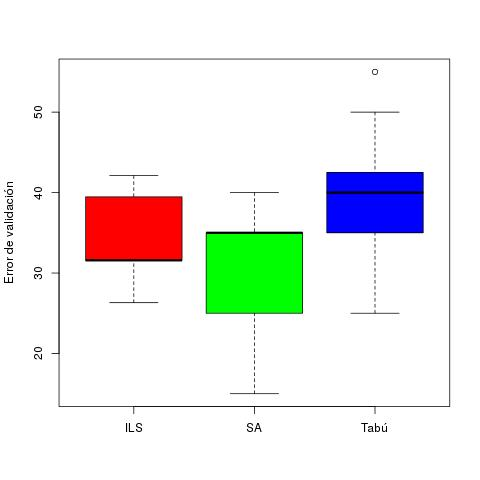
\includegraphics[scale=0.4]{val_errors.jpeg}~\\[1cm]
\end{center}

\begin{center}
  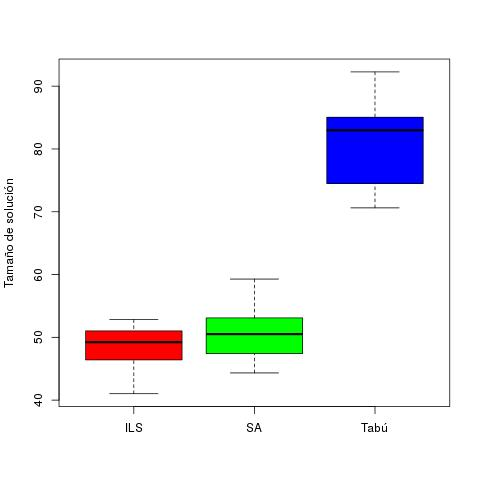
\includegraphics[scale=0.4]{sizes.jpeg}~\\[1cm]
\end{center}

% include your own bib file like this:
%\bibliographystyle{acl}
%\bibliography{acl2014}

\begin{thebibliography}{}

\bibitem[\protect\citename{Cano et al}2003]{Cano:03}
José Ramón Cano, Francisco Herrera, and Manuel Lozano.
\newblock 2003.
\newblock {\em Using evo-
lutionary algorithms as instance selection for data reduction in kdd: an
experimental study.}.
\newblock Evolutionary Computation, IEEE Transactions.

\bibitem[\protect\citename{Toussaint}200]{Toussaint:02}
Godfried Toussaing.
\newblock 2002.
\newblock {\em Proximity Graphs for Nearest Neighbor Decision Problem}.
\newblock School of computer science. McGill University

\end{thebibliography}

\end{document}
